\section{Ignorance Management}

There are numerous potential sources of ignorance when reasoning in the real world:
\begin{itemize}
    \item Insufficient data.
    \item Biased data: data collected by sensors affected by errors.
    \item Variable data: data collected by imprecise sensors.
    \item Reliability of data.
    \item Fuzziness.
    \item Reliability of the model: depends on the model design, implementation, and parametrization.
    \item Incompleteness of the model.
\end{itemize}
\begin{example}
    Let's consider the sentence "The elephant weighs 2 tons". This can be interpreted in various ways, each slightly different:
    \begin{itemize}
        \item The elephant weighs exactly 2 tons.
        \item The elephant weighs 2 tons $\pm$10 kg, given the resolution of the weight scales of the instrument.
        \item The elephant weighs approximately 2 tons, but we cannot say anything more precise.
        \item We are not sure about any previous sentence because we do not have enough evidence.
    \end{itemize}
\end{example}
\begin{figure}[H]
    \centering
    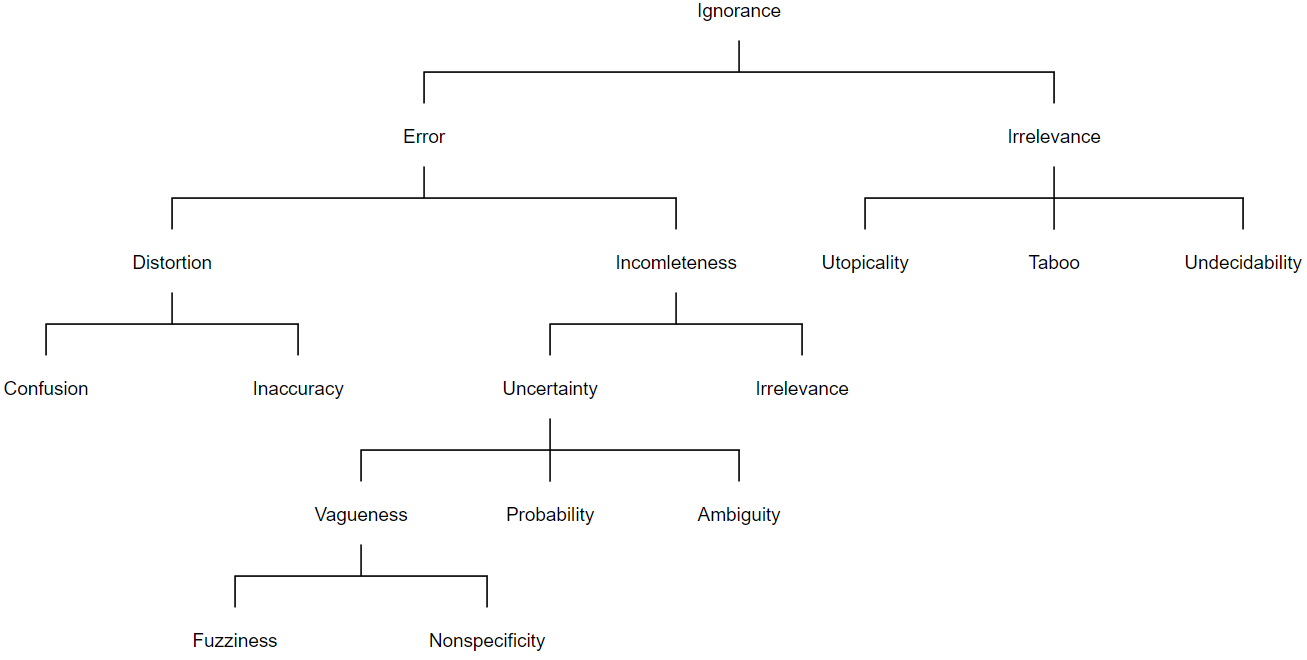
\includegraphics[width=0.75\linewidth]{images/smithson.png}
    \caption{Smithson's taxonomy of ignorance and uncertainty}
\end{figure}
To model ignorance, it is often decided to associate measures of certain aspects. Let's distinguish between two aspects:
\begin{itemize}
    \item The type of representation: numbers, labels, intervals, etc.
    \item The represented ignorance that we would like to model, such as probability, reliability, subjective evaluation, etc.
\end{itemize}

\paragraph*{Probability}
Probability is represented with numbers between zero and one, and a well-established set of rules and properties are associated with its management. For example:
\begin{itemize}
    \item The sum of probabilities should equal one.
    \item The probability a posteriori of a hypothesis $h_i$ given some evidence $e$ is given by the Bayes theorem:
        \[\textnormal{P}(h_i \mid e)=\dfrac{\textnormal{P}(e \mid h_i)\textnormal{P}(h_i)}{\textnormal{P}(e)}\]
\end{itemize}

Probability has been used in applications like MYCIN, one of the first expert systems designed for diagnosing blood illnesses. 
MYCIN modeled certainty by considering two numerical factors:
\begin{itemize}
    \item Measure of increased Belief: 
        \[\textnormal{MB}=\dfrac{\textnormal{P}\left(\frac{h}{e}\right)-\textnormal{P}(h)}{1-\textnormal{P}(h)}\]
    \item Measure of decreased Disbelief: 
        \[\textnormal{MD}=\dfrac{\textnormal{P}(h)-\textnormal{P}\left(\frac{h}{e}\right)}{\textnormal{P}(h)}\]
\end{itemize}
The measure of a statement is given by the certainty factor:
\[\textnormal{CF}=\textnormal{MB}-\textnormal{MD} \in [-1;1]\]

A key hypothesis for this solution is that the numbers given as $\textnormal{MB}$ and $\textnormal{MD}$ are not statistical probabilities but subjective probabilities, provided by different experts and combined using rules (which can introduce ambiguity).

In comparison to probabilities, linguistic terms are less ambiguous than numbers. 
Using a limited set of labels, it is possible to associate subjective evaluations with statements, making it relatively easy to achieve consensus on subjective judgments. 
A computational mechanism is then needed to define how to combine labels. 
This is achieved through the use of fuzzy systems, which represent the truth of a statement in linguistic terms and evaluate its fuzziness.